\documentclass[11pt,a4paper,oneside]{article}
\usepackage{graphicx}
\usepackage[section]{placeins}
\usepackage{hyperref}
\hypersetup{
    colorlinks,
    citecolor=blue,
    filecolor=blue,
    linkcolor=blue,
    urlcolor=blue
}
\usepackage[all]{hypcap}

\begin{document}
\begin{titlepage}

\begin{center}


\includegraphics[width=1\textwidth]{images/sponsor-logo.png}\\[1cm]    

{ \huge \bfseries Project Plan}\\[0.4cm]
{ \large \bfseries Infographic Generator}\\[0.4cm]

Louis Bodnar\\
Peter Chen\\
Lok Cheung\\
Kevin Shreve\\



\vfill

{\large \today}

\end{center}

\end{titlepage}

\tableofcontents

\newpage

\listoffigures

\newpage

\section{Executive Summary}


The Infographics generator will create a new an intuitive way to present the Key Performance Indicators (KPI) that Urban Science has been collecting. Our HTML5 mobile application will be used to show Corporate OEM’s or Ford plant managers, the exact kind of data to improve performance.\\

The main objective of this system is to increase usage of the KPI data, and make it easier to read and understand. Users will be able to use a selection screen to find a category in which they have interest. Once a category is selected, the following screen will bring up an infographic containing data related to that category. This functionality will allow the user to easily find the infographic they want to see. Urban Science is in a great market position, where in bad economic times companies use their data to save money, and in good economic times companies use Urban Science to help them make money. Our application will deliver a robust solution to break down the data, so that clients can know exactly what relevant data in order to be successful.\\

Our software will also build the framework to allow Urban Science to continue to use our product, by being able to easily add in more infographics. This allows for future extensibility for Urban Science to keep the similar look and feel that the users will become accustomed to seeing. This product will be a key selling point for Urban Science to offer its clientele as the easy to understand interface will guide their customers towards new goals.\\


\section{Functional Specifications}

The main focus of project is to create a new and creative experience for the KPI data. The user interface will be very simple, allowing for on the fly use by those giving presentations or demonstrating the product to clients. When a client sees this unique display of information they will assuredly choose Urban Science to help them with their strategy.\\

The system will be a standalone web app, but may have the possibility of being pulled into another website at their discretion. It will be displayed via Safari on an iPad, with the android platform or access via a desktop computer being the secondary access point.\\


\section{Design Specifications}

\subsection{Overview}
% TODO replace default graph

The general interface is based on a Lazy Susan like menu. A user can swipe the screen to rotate the icons, and just touch on anyone of them to select a category. The program will trigger the infographic generator depending on the category that was selected. The infographic generator will then grab the preloaded data from the xml file and display with a default graph. Then user can select different style of infographic to display the information as they need.\\

\begin{figure}[!]
\caption{Use Case Diagram}
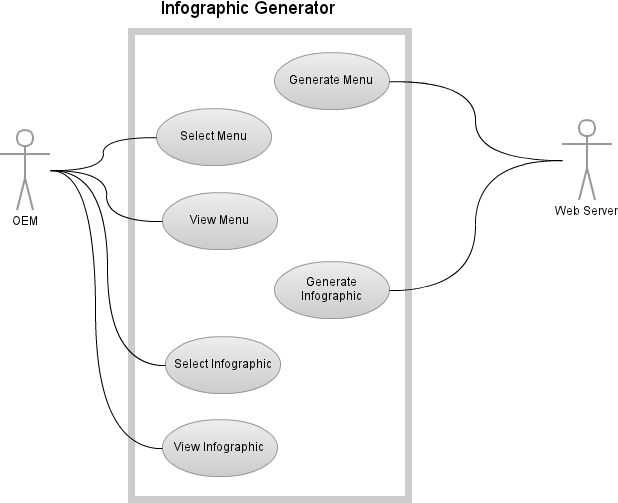
\includegraphics[width=1\textwidth]{images/Capstone_-_Use_Case_Diagram.png}\\   
\end{figure}


\subsection{System Architecture}

The infographic application is comprised of two major components: a web application/user interface and a backend database. Users are assumed to use safari browser on iPad. The web host then displays the menu screen. Data will be pulled until specific category is selected. When a category is selected, the program will pull up all the required data from the server. Depending on the style of infographic, data will be displayed in different form.\\

\subsection{User Interface}

Figure~\ref{mockup-main-menu} shows the screen mockup for our prototype.  The main page will be displayed in lazy Suzan style that allows the user to scroll through the icons to the right or left.  The infographic for the current category will be shown when the icon is clicked on.\\


Figure~\ref{mockup-infographic-display-1}, Figure~\ref{mockup-infographic-display-2}, and Figure~\ref{mockup-infographic-display-3} show a sample infographic depiction.  If you want to view data for another month, you can just swipe left and right to change the time frame.  If you want to go back to the main menu page, just click on the top right corner’s menu button.\\


\begin{figure}[!]
\caption{Main Menu Mockup\label{mockup-main-menu}}
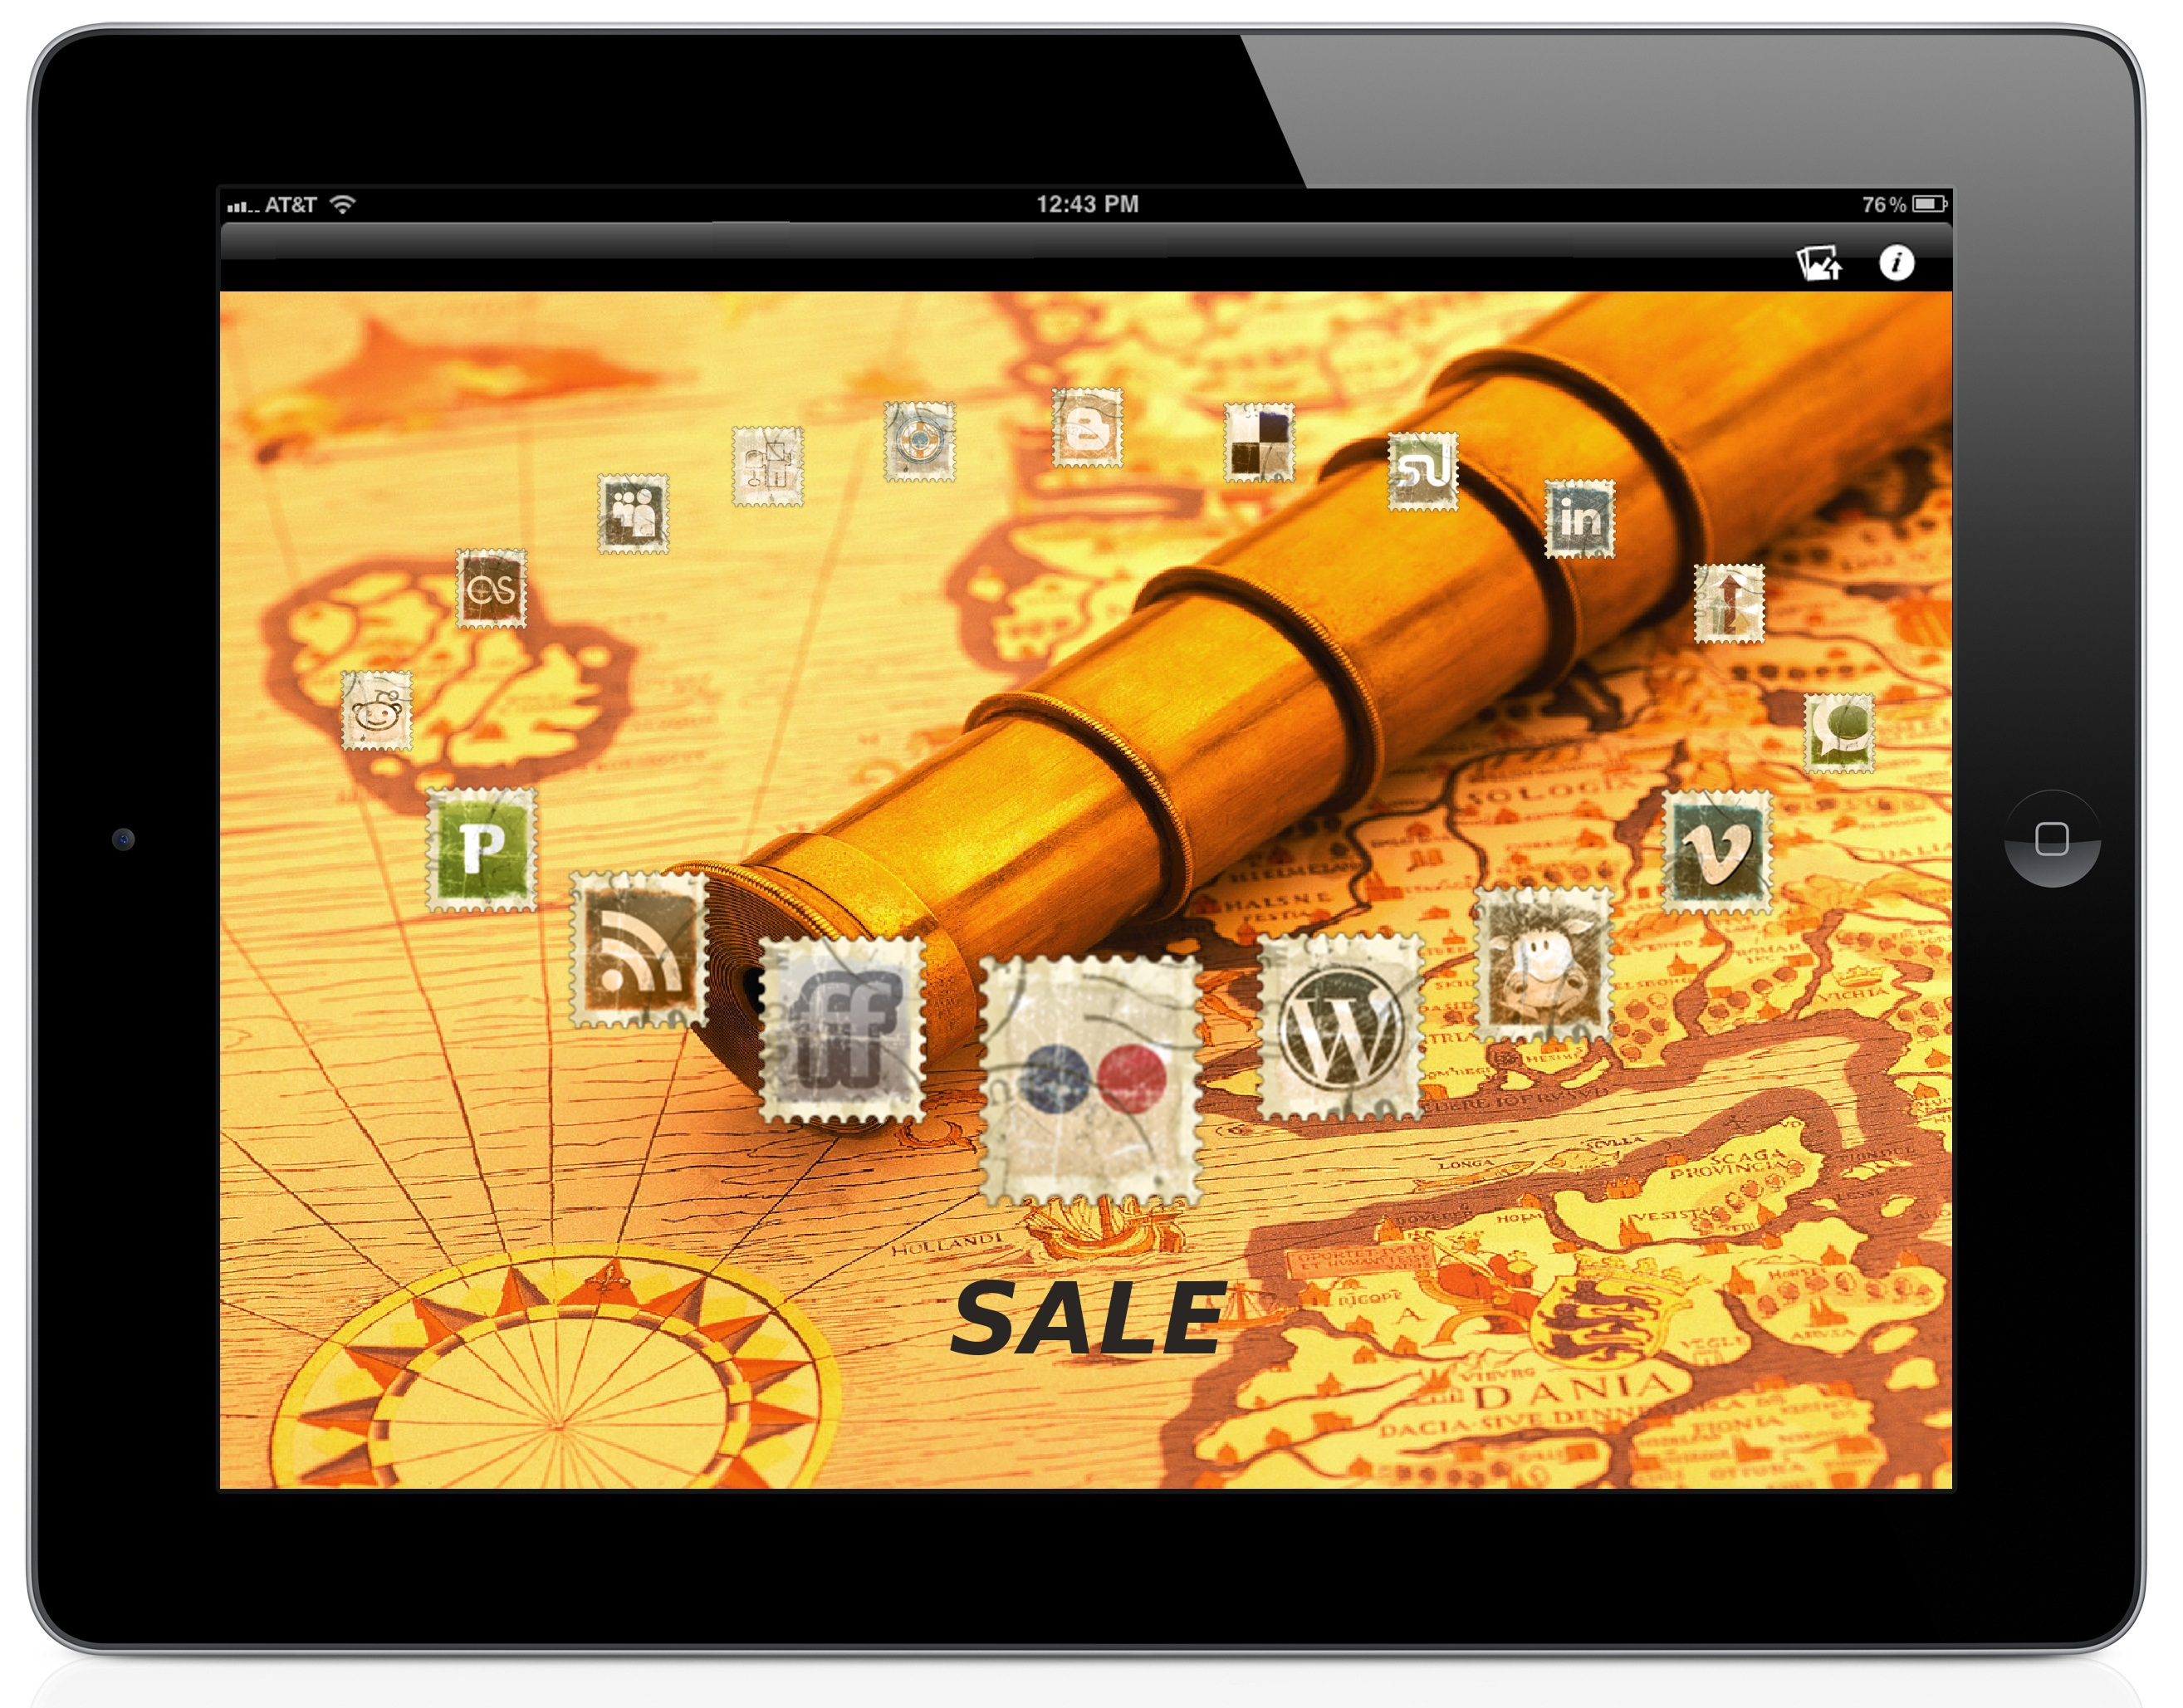
\includegraphics[width=1\textwidth]{images/screen.jpg}\\
\end{figure}


\begin{figure}[!]
\caption{Infographic Display Mockup\label{mockup-infographic-display-1}}
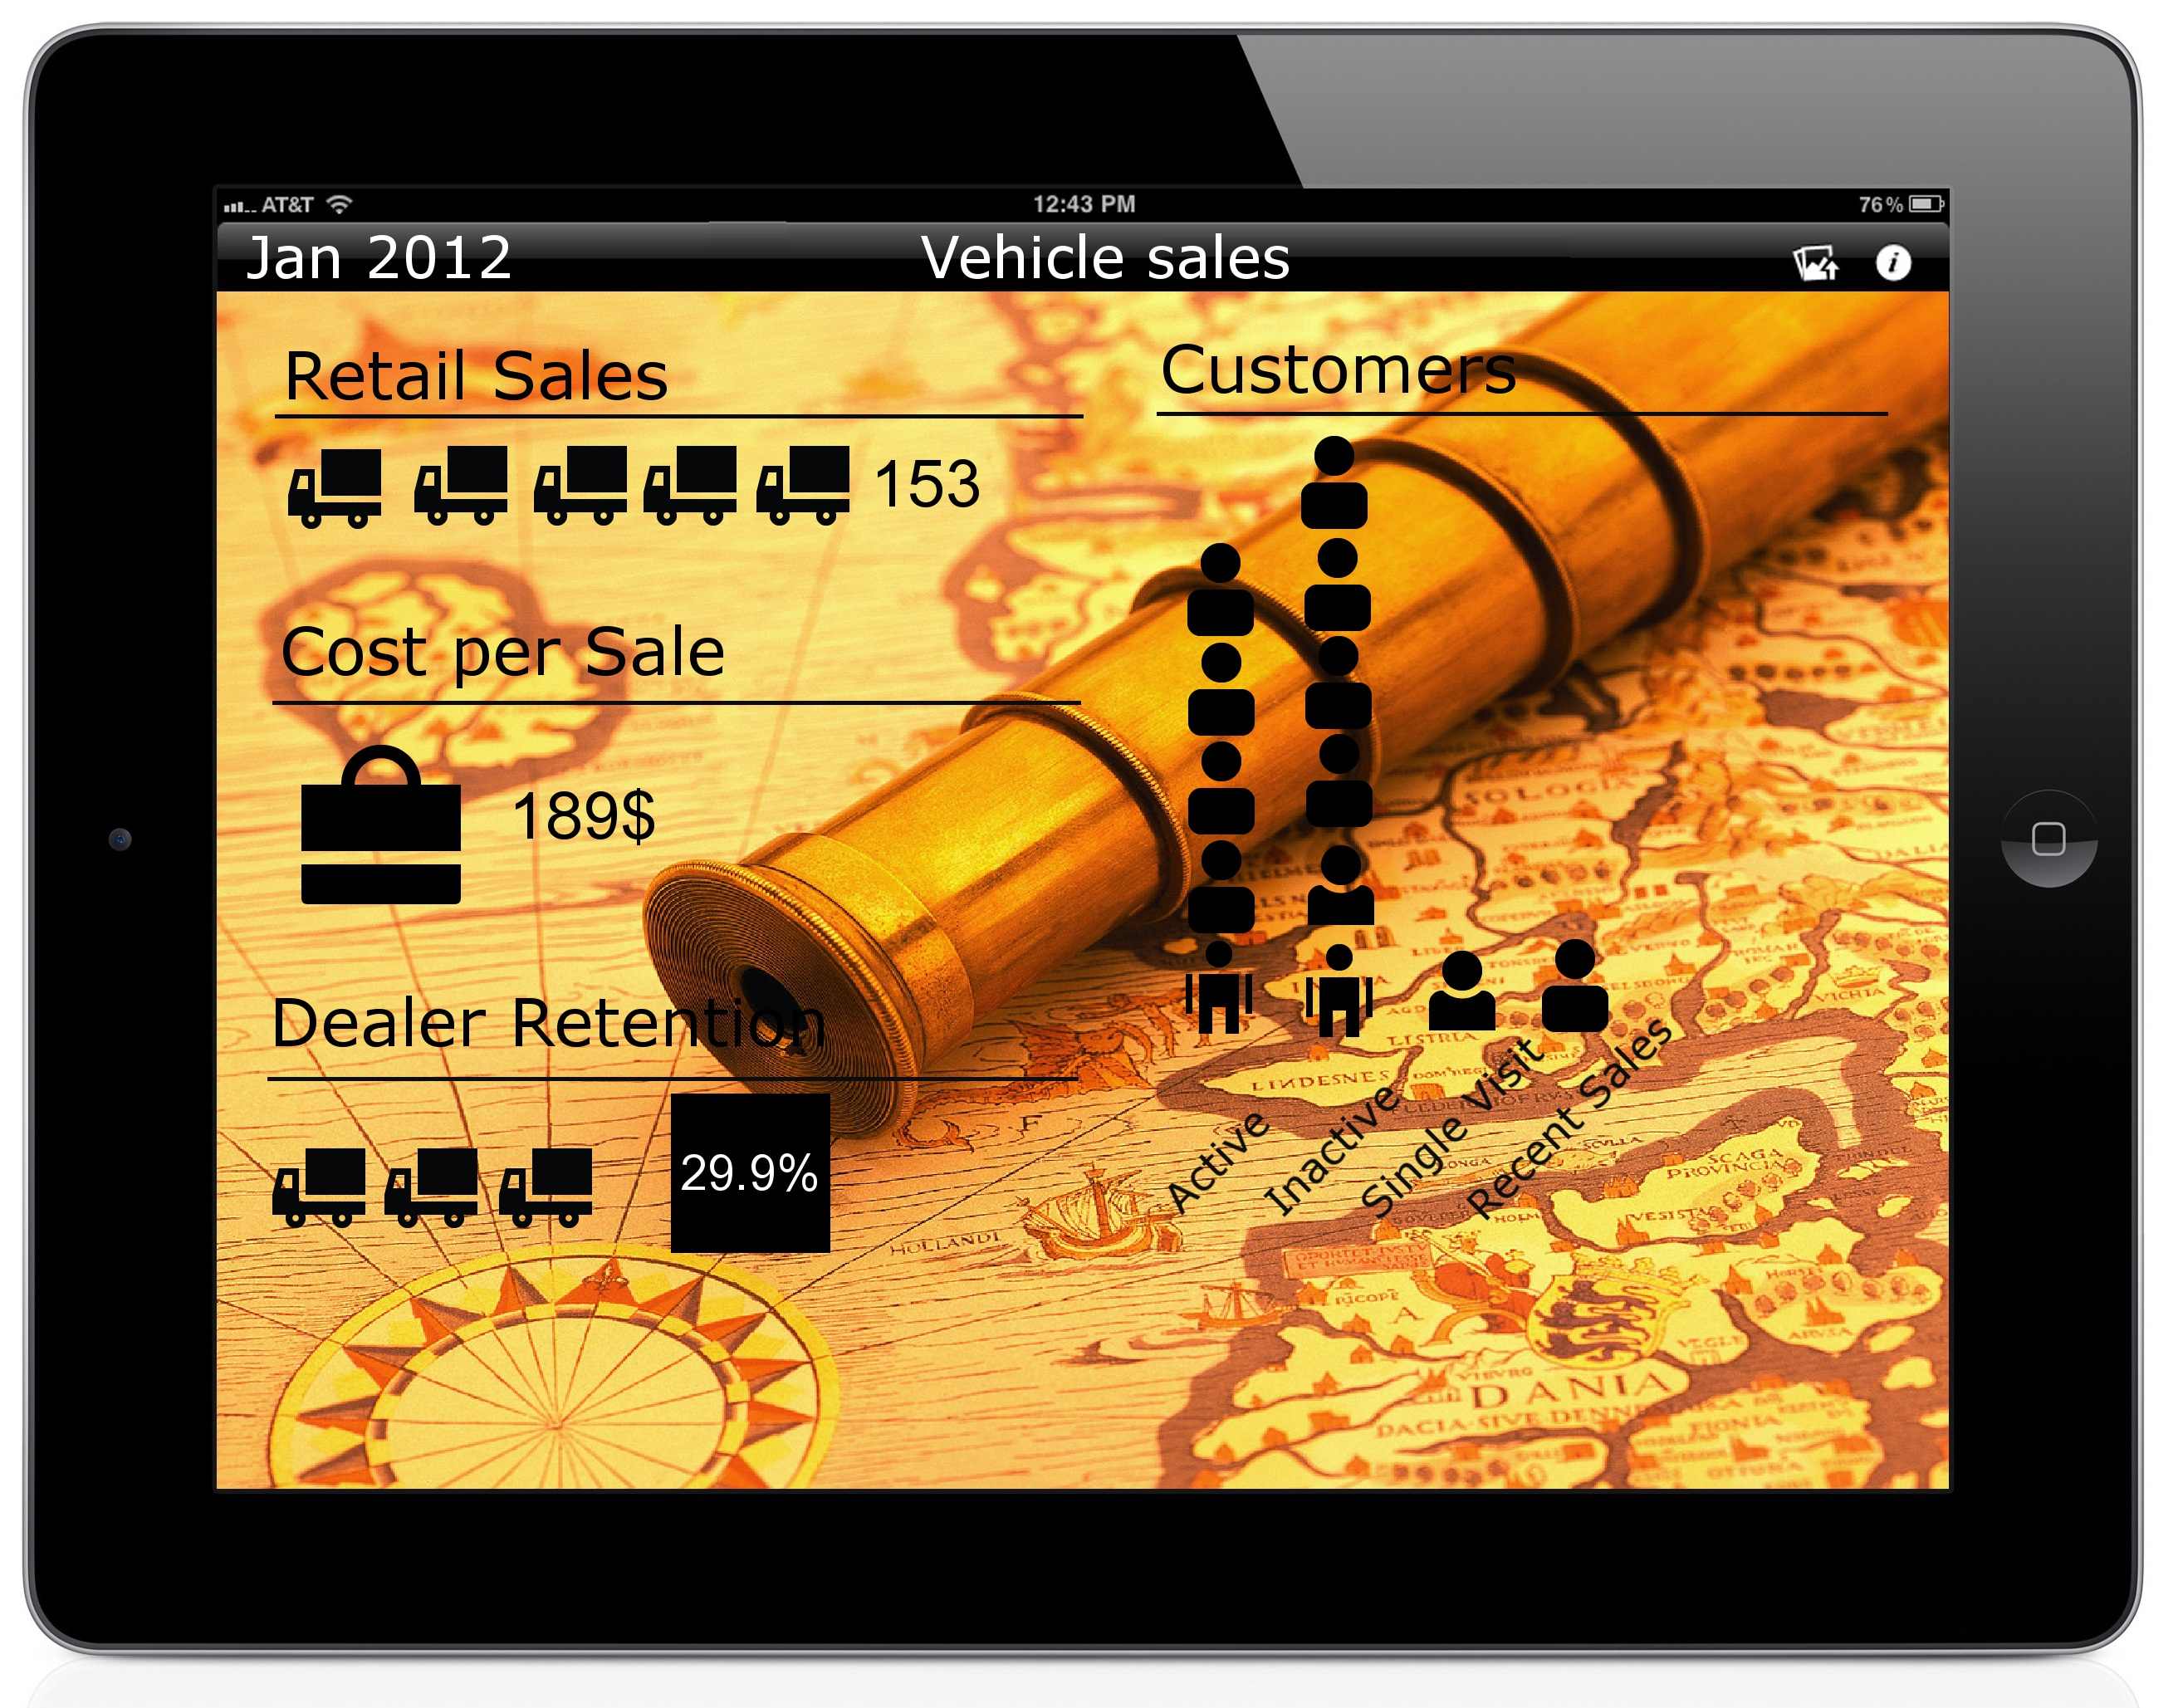
\includegraphics[width=1\textwidth]{images/screen5.jpg}\\
\end{figure}

\begin{figure}[!]
\caption{Infographic Display Mockup\label{mockup-infographic-display-2}}
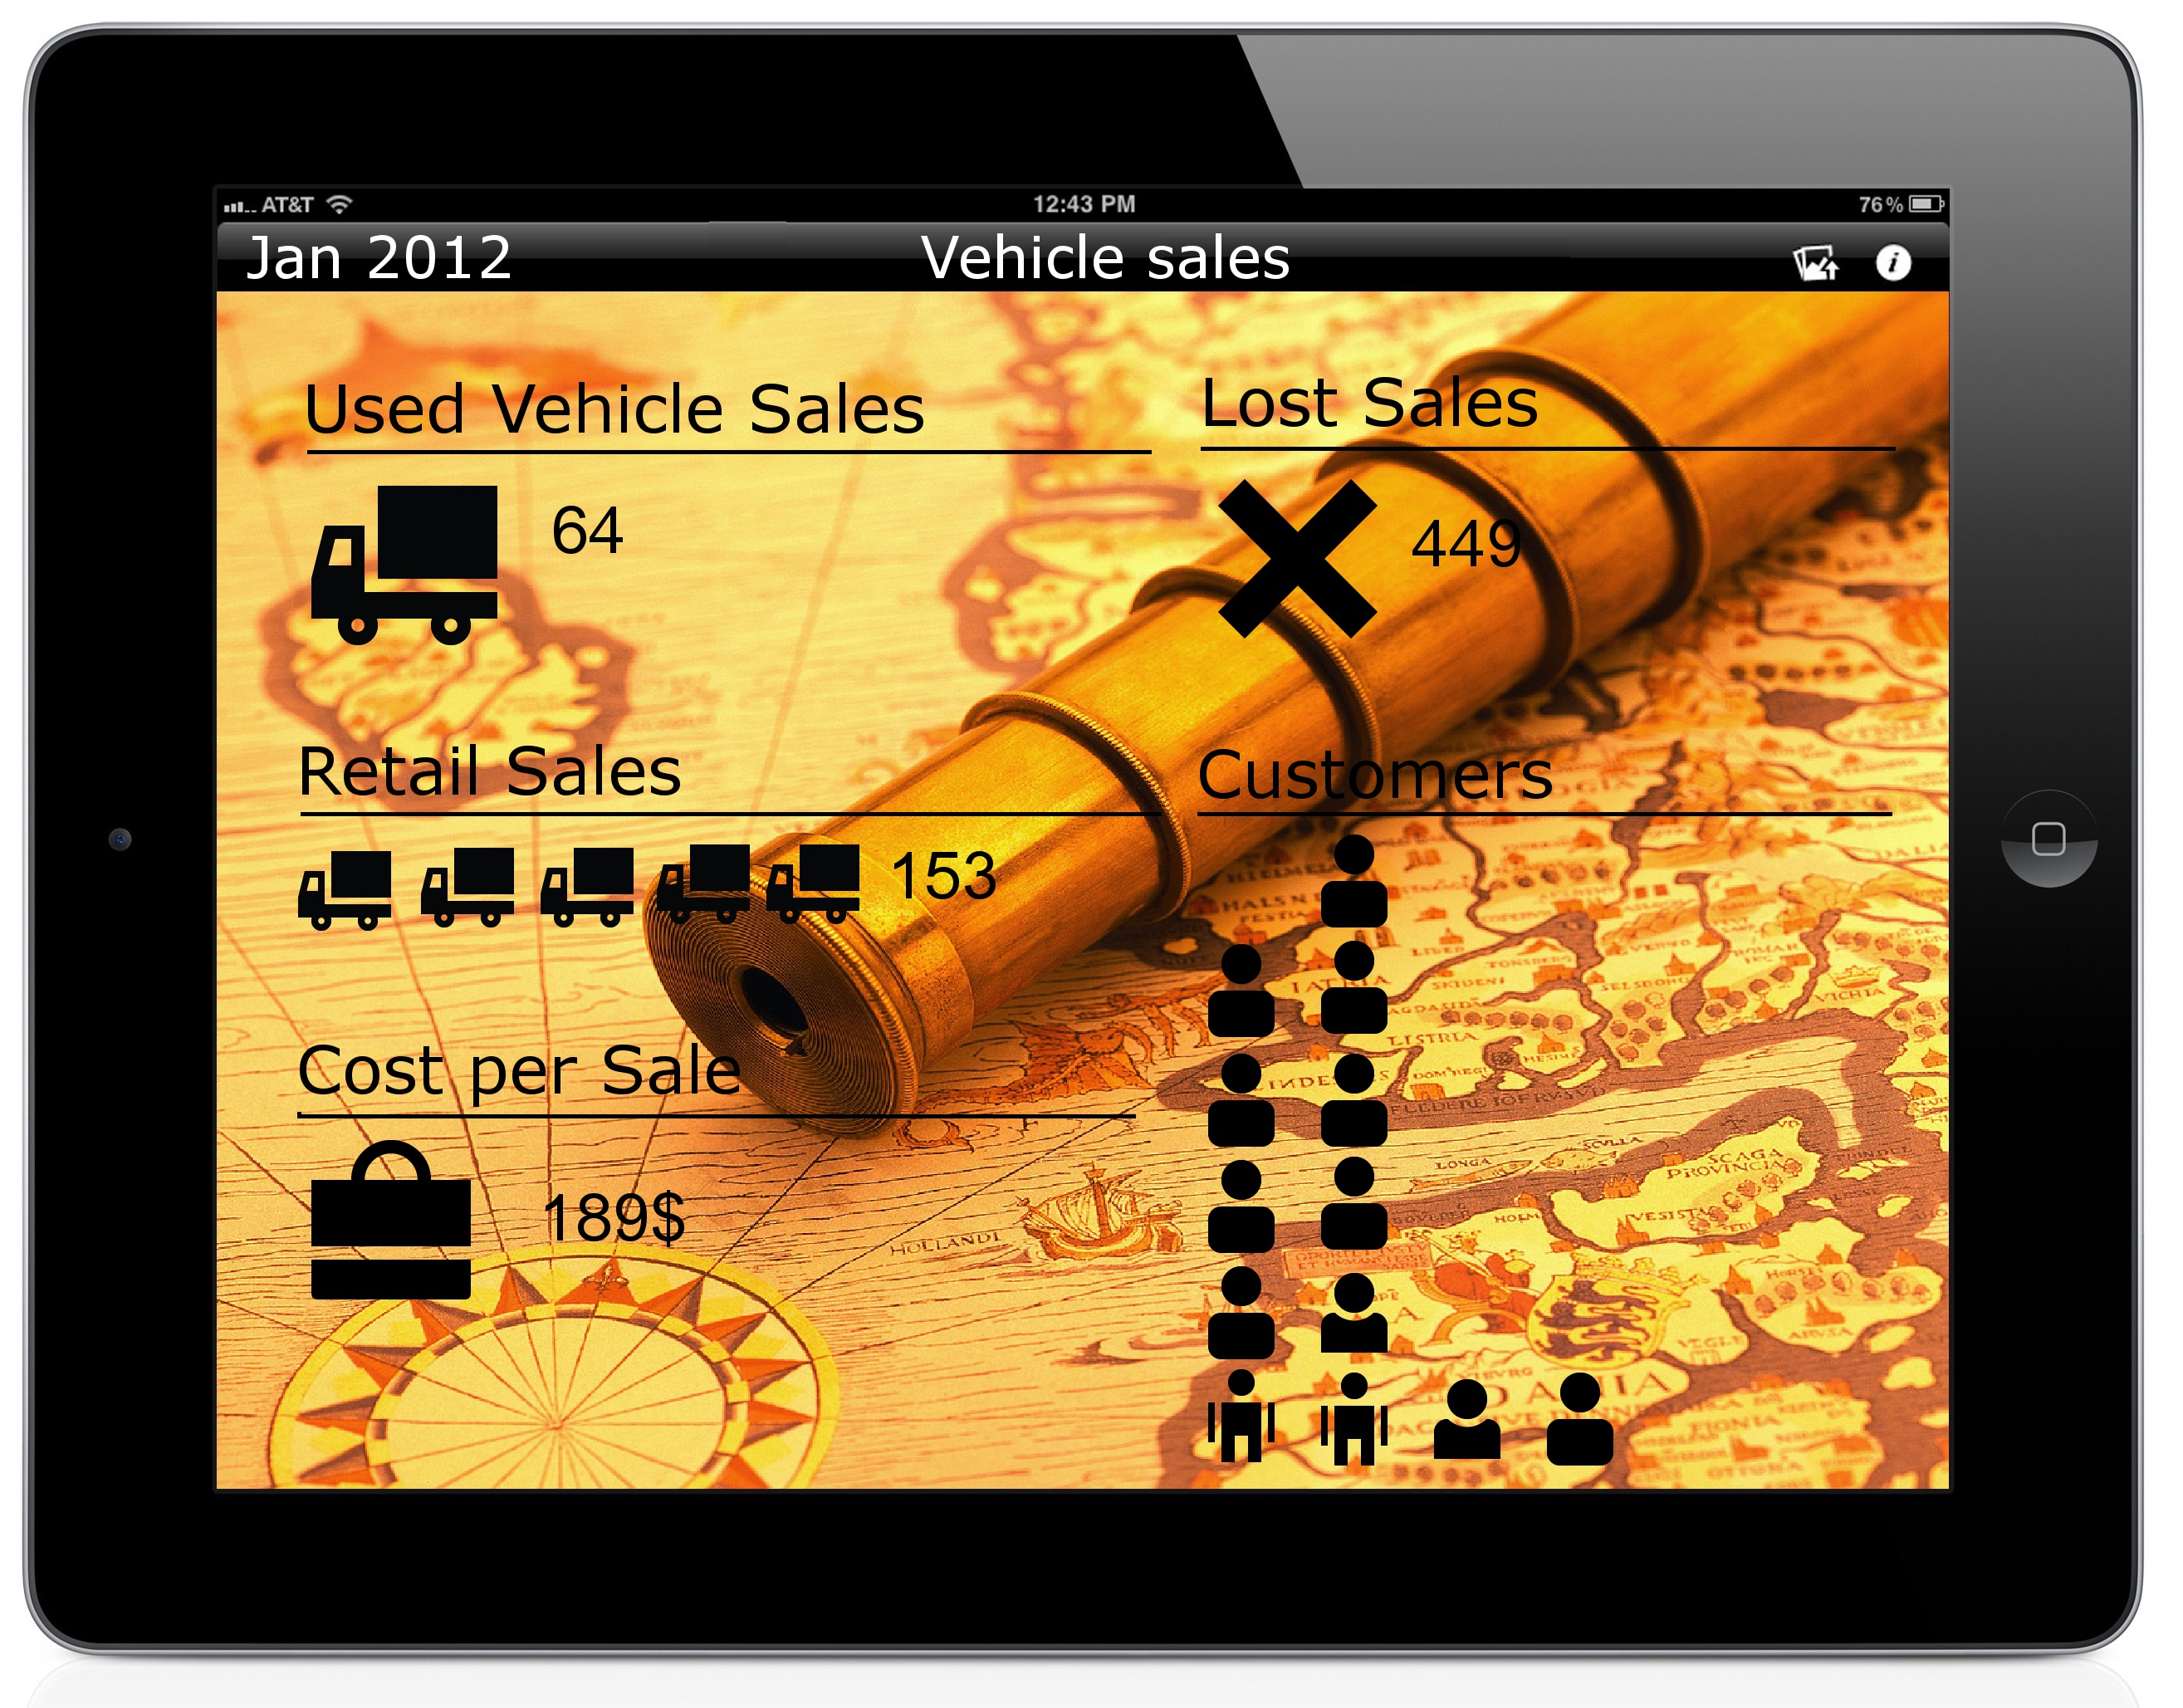
\includegraphics[width=1\textwidth]{images/screen3.jpg}\\
\end{figure}

\begin{figure}[!]
\caption{Infographic Display Mockup\label{mockup-infographic-display-3}}
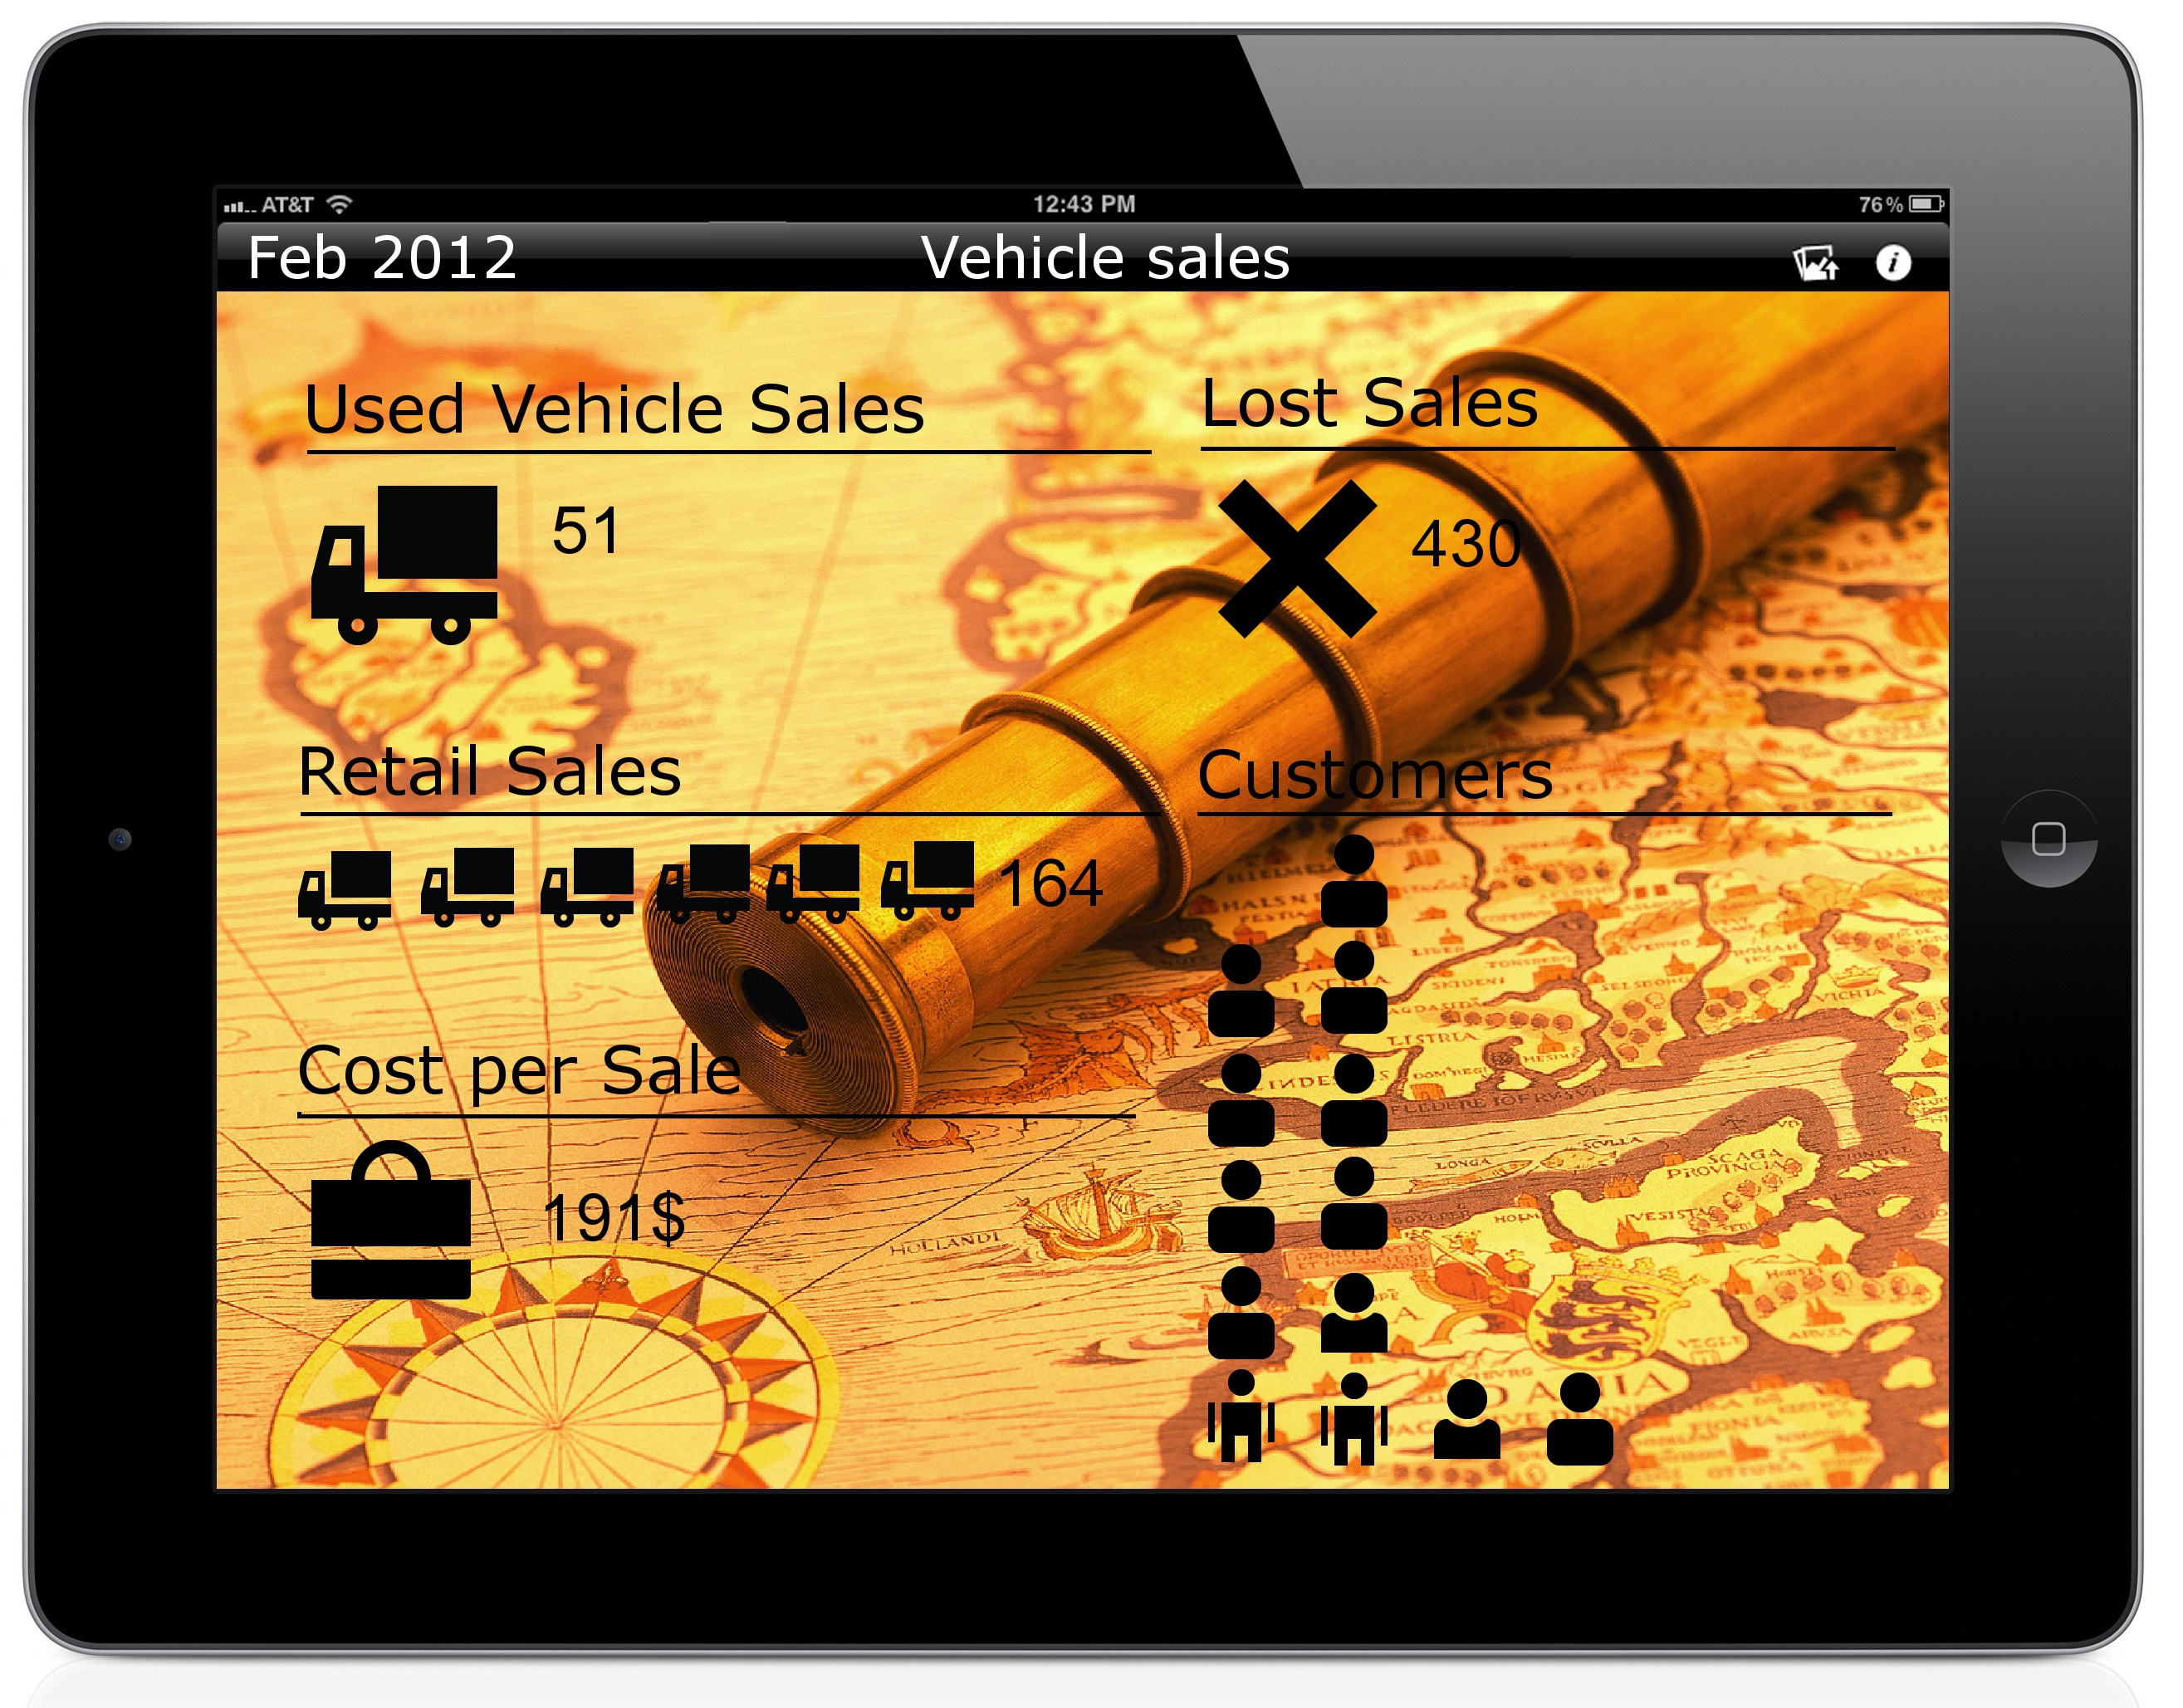
\includegraphics[width=1\textwidth]{images/screen4.jpg}\\
\end{figure}

\section{Technical Specifications}

The infographic generator will produce infographics suitable for display in a browser with support for HTML5 and JavaScript.\\


Each infographic will be based off of KPI data returned from a Microsoft SQL database.  The server will use an asp.net script to query the database and return the information to the client device.  The client device will integrate this data with predefined infographic scripts written in a combination of HTML5 and JavaScript to generate the infographic.\\


An infographic framework consisting of the server side database query script and a client side JavaScript library will be used to assist in the creation of infographics.  The JavaScript library will contain functions to create reusable animations and artwork based off values obtained from the database query script.\\


The interface for viewing infographics will be written in HTML5 and JavaScript.  It will use jQuery to support swipe events on the iPad for scrolling left and right in the menus.  The menus will be populated with items read from an XML file.  Only the front most item (the item with the greatest cascading style sheet z-index) in the menu will be selectable.  The front most item will change to the item on its immediate left if swiped right and vice-versa if swiped left.\\


The main menu will be used to select a category.  Once the category has been selected, the contents screen will change to show the infographic for the selected category.  The user will have the ability to return to the main menu while viewing an infographic.  This functionality will be provided by a button located on each infographic display page but not as part of the main menu.\\

\begin{figure}[!]
\caption{Sequence Diagram}
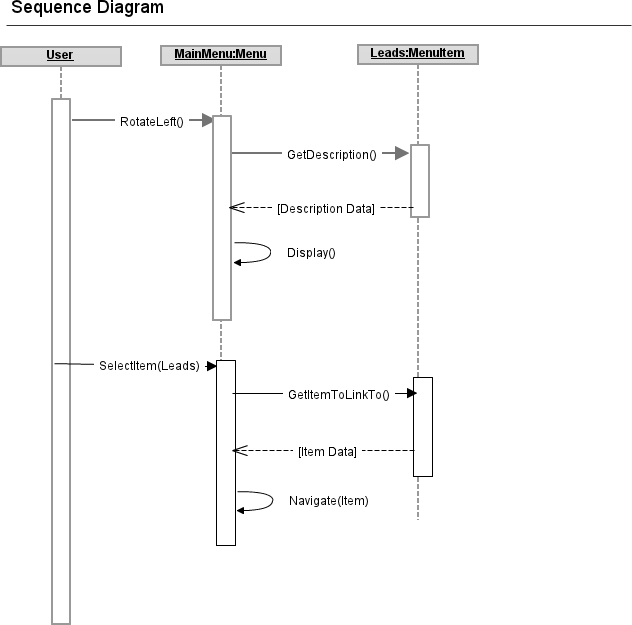
\includegraphics[width=1\textwidth]{images/Capstone_-_Sequence_Diagram.png}\\
\end{figure}


\begin{figure}[!]
\caption{Class Diagram}
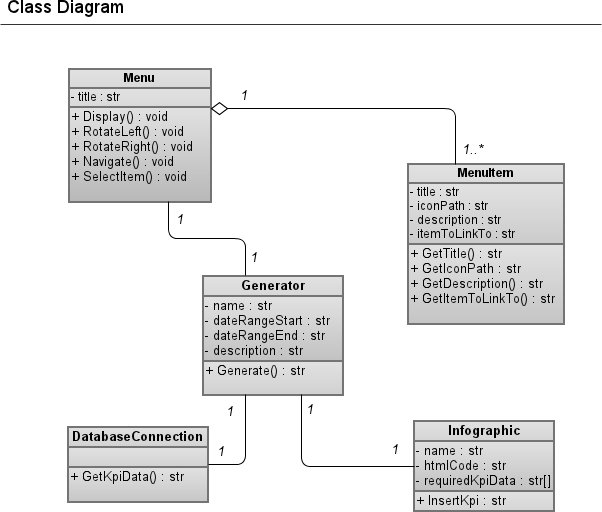
\includegraphics[width=1\textwidth]{images/Capstone_-_Class_Diagram.png}\\
\end{figure}


\section{Schedule}

\subsection{Week 1 (Jan 9 - Jan 15)}
\begin{itemize}
\item Had our first conference call with our customer
\item Set up weekly conference calls with our customer
\item Set up regular team meetings to meet twice a week
\item Installed virtual machines
\end{itemize}


\subsection{Week 2 (Jan 16 - Jan 22)}
\begin{itemize}
\item Started UML diagrams
\item Installed Windows Server 2008 R2
\item Installed IIS 7
\item Installed ASP.NET
\item Installed Microsoft SQL Server
\item Talked with our customer about interface mockups
\end{itemize}

\subsection{Week 3 (Jan 23 - Jan 29)}
\begin{itemize}
\item Completed more UML diagrams
\item First draft of project-plan
\item Installed Visual Studio 2010
\item Created screen mockups
\item Created sample infographic elements
\end{itemize}

\subsection{Week 4 (Jan 30 - Feb 5)}
\begin{itemize}
\item Created infographic elements using actual KPI data
\item Wrote website to showcase infographics
\item Decided to work on sales infographic first
\end{itemize}

\subsection{Week 4 (Feb 6 - Feb 12)}
\begin{itemize}
\item Presented project plan to class
\item Changed from using XML to JSON for pulling database information
\item Have roundabout working with several images for infographic selector buttons
\item Successfully pulled data from a SQL database using ASP.NET
\end{itemize}


\section{Risks}

\subsection{Languages}

\begin{itemize}
\item Risk: Unfamiliar with ASP.NET and HTML5 
\item Mitigation: Read online tutorials, books, and documentation
\end{itemize}


\subsection{Ambiguous Requirements}

\begin{itemize}
\item Risk: Customer gave broad requirements
\item Mitigation: Help customer find focus by using mockups and eliciting information
\end{itemize}


\subsection{Scheduling}

\begin{itemize}
\item Risk: Not much free time overlap between our schedules
\item Mitigation: Keep everybody up-to-date with emails and plan ahead
\end{itemize}


\subsection{Art}

\begin{itemize}
\item Risk: Little artistic experience in our group
\item Mitigation: Brainstorm and find inspiration from the artwork used in popular applications
\end{itemize}




\end{document}
